% 4-7 题 图4_5：匀质圆环绕水平轴转动，轴下移至地面
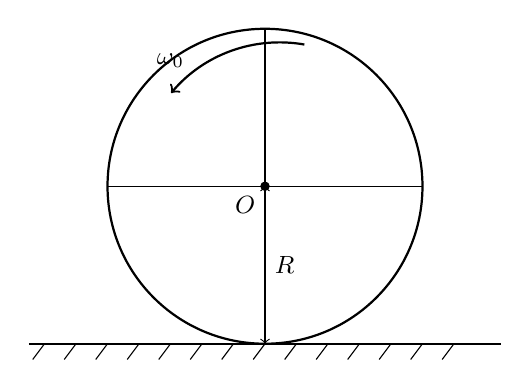
\begin{tikzpicture}[font=\small]
  % 圆环
  \draw[thick] (0,0) circle (2);
  % 辐条（十字形）
  \draw[thin] (-2,0) -- (2,0);
  \draw[thin] (0,-2) -- (0,2);
  % 中心轴标注
  \filldraw (0,0) circle (1.5pt) node[below left] {$O$};
  % 角速度箭头（圆弧箭头）
  \draw[->, thick] (0.5,1.8) arc[start angle=80, end angle=140, radius=1.8];
  \node at (-1.2,1.6) {$\omega_0$};
  % 水平地面线
  \draw[thick] (-3,-2) -- (3,-2);
  % 地面阴影
  \foreach \x in {-2.8,-2.4,...,2.8} {
      \draw (\x,-2) -- (\x-0.15,-2.2);
  }
  % 标注 R
  \draw[<->] (0,-2) -- (0,0) node[midway, right] {$R$};
\end{tikzpicture}
